
\documentclass[letterpaper,12pt]{report}
\usepackage{thesis}
\usepackage[toc,page]{appendix}
\usepackage{adjustbox}
\usepackage{hyperref}
\usepackage{listings}
\usepackage{url}
\usepackage{lipsum}
\usepackage{courier}
\usepackage{tabu}
\usepackage{algorithmic}
\usepackage{amsfonts}
\usepackage{tcolorbox}
\usepackage{geometry}
\usepackage{multirow}
\usepackage{enumitem}
\usepackage{float}
\geometry{%
letterpaper, % a4paper
left=   20 mm,
right=  20 mm,
top=    15 mm,
bottom= 20 mm,}
%\usepackage{setspace}
%\doublespacing
\usepackage{amsmath}
\usepackage[T1]{fontenc}
\usepackage{titlesec}
% various other packages
\titleformat{\chapter}
  {\normalfont\Large\bfseries}{\thechapter}{.5em}{\vspace{.5ex}}[\titlerule]
\titlespacing*{\chapter}      
    {0pt}{0pt}{15pt}
\usepackage{caption}
\usepackage{amssymb}%
\setcounter{MaxMatrixCols}{30}%
\usepackage{graphicx}
\usepackage{algorithm}
\usepackage{pgfplots,pgfplotstable}
\usepackage{filecontents}

%\usepackage{algpseudocode}
\usepackage{pifont}
\providecommand{\U}[1]{\protect\rule{.1in}{.1in}}
%EndMSIPreambleData
\begin{document}

\pagenumbering{roman}

% Fill in the title, author, degree name, department, and month/year.
% Upon completion, this should look like the following:
%\thesistitle
%	{Complicated and Important-Sounding Thesis Title}
%	{John P. Doe}
%	{Master of Science}
%	{Department of Computer Science}
%	{May 2009}
% The \thesistitle definition is in thesis.sty.  Other customizations
% can be made there.
\thesistitle
{
	 Clowder:  Software for Managing Cluster Of High Performance Computers  }
	{\emph{Samson Ugwuodo}}
	{Master of \emph{Science}}
	{ \emph{Scientific Computing} Program}
	{\emph October 2017} 

\addcontentsline{toc}{chapter}{Abstract}
\begin{center}
\textbf{\large Abstract}
\end{center}

Clowder is a system designed to help researchers in the Faculty of Engineering and Applied Science to manage and control clusters of test machines. Some of the features that required improvement in this system were the ability to reserve a machine for a certain period of time, a function that allows users to add more computers and manage their properties, and a user interface where users can have interactive access to the system. Therefore, there was a need to upgrade and complete this system by developing software that provides the  missing functionality. A web interface improves the user accessibility. Having a dynamic database system provides the functionality of keeping record of user activities, storing computer information and managing all reservations. These design approach were achieved using SQL models, HTML templates and the Go programming language. Instead of performing several command line prompt statements, which is the current method in the use of Clowder system, the software provides flexible user access to the cluster of computers, a dynamic system management in a single software system as a research tool in the Faculty of Engineering and Applied Science.    

\hfill

\addcontentsline{toc}{chapter}{Acknowledgements}
\begin{center}
\textbf{\large Acknowledgements}
\end{center}

 \begin{center}
\begin{center}
\begin{flushleft}
I will like to express my humble thanks to my supervisor Dr. Jonathan Anderson for his overwhelming support, guidance, professional advise as a professor and his contribution through out this project.  
 
I want to express my sincere appreciation to the School of Graduate Studies, the Department of Scientific Computing and Computer Engineering for their academical and financial support.
 
I would also like to thank the head of Department Dr Ronald Haynes , and Gail kenny for their subsequent advice and support through out my in class academic works and other wise.
 
Finally, I am grateful to my family and God almighty for the love and encouragement that i have been blessed with through out this journey.
\end{flushleft}
\end{center}
 \end{center}

\hfill 

\tableofcontents

\addcontentsline{toc}{chapter}{List of Tables}
\listoftables

\addcontentsline{toc}{chapter}{List of Figures}
\listoffigures

\pagenumbering{arabic}
\chapter{Introduction}
\label{chap:intro}

The use of high performance computers for  research in the Faculty of Engineering  and Applied Science has increased, because of increase in research tasks, such as testing new operating systems. As researchers demand robust computers, these computers systems also need to be expanded to accommodate these large tasks. As we expand the systems, access and usage  becomes more complicated to manage. Therefore we are faced with issues of system management, system accessibility, and storage. These issues are the inability to provide  a proper record of each computer system and its usage, the inability to provide flexible user access to the computers, and also the problem of monitoring the number of computers that are reserved by users. As a result of these challenges it is necessary to develop software that solves these problems for the Faculty of Engineering and Applied Science. 


Clowder is a system designed to provide a Preboot Execution Environment (PXE) for testing new operating systems through a Network File System (NFS) sever. Others have worked on this system for several years, but there was more work yet to be done to improve its existing features and functionality. As an example, it takes manual command line statements to access  a computer in the cluster during research. Another reason for improvement is to provide flexible and dynamic user interface rather than the current manual, error-prone norm (SSH). Therefore the current state of Clowder is not flexible and convenient enough. So the main goal of this project is to develop software that addresses the issue of user accessibility, system management and automatic control protocol. Addressing all these issues will improve the performance of Clowder in speed, access and robustness, making it a complete software tool. 
	
	
We have accomplished this goal by using a design approach that augments a previously existing interface and database system. The database system is designed to store and keep record of the computer systems and user activities. The web interface enable users to have access to the Clowder system from different locations simultaneously via a web page, and also provides users with the system inventory and other user activities. This  software provides the ability to search for data in the inventory, and to add new computer systems to the cluster, and to modify their properties individually. Also it provides the ability to make reservations: to allow users to reserve a computer for a certain period of time, and to end reservations as well.    
	

As this software serves as a tool to manage the cluster of computers and user activities, it is important to know that  reservations made, computer details, network interface cards and disks are stored as data. So all the computer system installed in the cluster with their names, vendors, memory size, architecture, and microarchitecture is stored in the database. The same is applicable to the disks, network interface cards and any other devices that could be part of the cluster. Data is represented as variables in their various data types in the database scheme.  All this information stored in the database tables serves as input  data for the program. This database scheme allows user to add or update new machines installed in the cluster, and therefore provide data record for the inventory on the web interface. 

The web interface serves as a platform for users to interact with the system and overview other users' activities via a web page. This interface can also  partially replace the SSH accessible command line prompt which was the previous user interface for Clowder system. This choice provides flexible access to and control of the system, by allowing users to log on to the system and make requests of the inventory at any time through the web server.
\autoref{Designofprogram} shows a general description of the Clowder system.

\begin{figure}[h]
  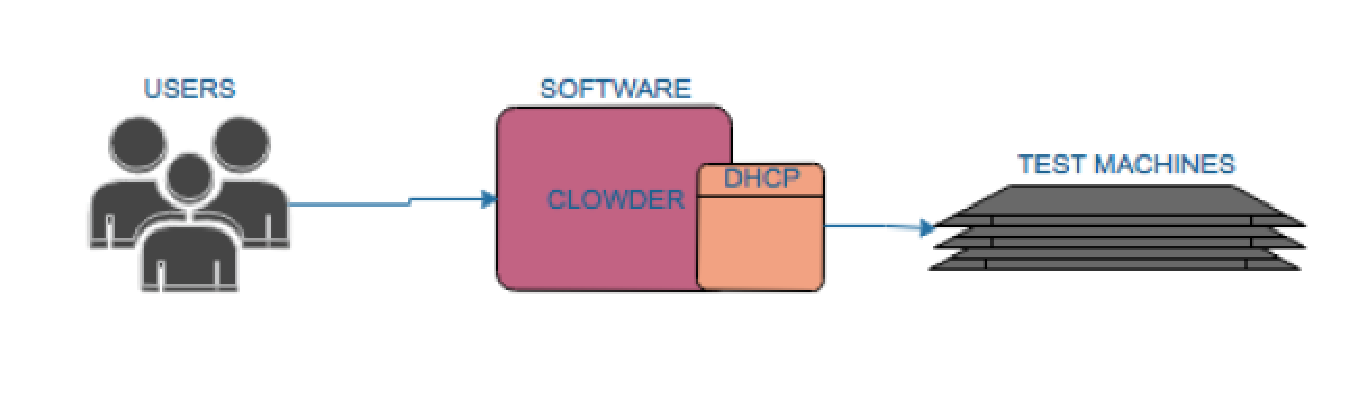
\includegraphics[width=\linewidth]{background.eps}
  \caption{A general design of the system}
  \label{Designofprogram}
\end{figure}
\pagebreak

This figure showcases the background concept of the Clowder as a full system. This concept is shown in detail in Fig 3.1, which explains the software functionality and data flow between the user interface and database. Following this chapter, we explain in more detail about the background of this system and other components that made up the design.

\section{Contribution}
I have contributed to this project to improve its existing interface and database functionality in other to have Clowder as complete software tool. My work includes the addition of required features to the interface such as; searching data from the system inventory, making reservation, checking for available machines, updating the system data, filtering and sorting the system inventory. These features were extended to the database improve its existing functionality. I have further explained this contributions in section \ref{Designstructure} and section \ref{Programstructure}.

\chapter{Background}
\label{chap:figtab}
\label{chap}
\section{Clowder}
Clowder is made up of various components, and some of these components have been worked on by researchers in the department. The goal of this project is to complete the Clowder system by developing the remaining components, which are to solve the issue of user accessibility and system management. Generally Clowder has been designed to manage access of cluster of test machines, mainly for testing new operating systems. But as this requires a flexible user interface and database to complete this components, we have improved the existing user interface by adding a dynamic web interface which is extended to the back end with more functionality. The background components of Clowder includes  a  DHCP server with Preboot Execution Environment (PXE)  that allow the test machines to be boot up remotely by users for testing. The test machines do a PXE boot and by using the DHCP to get IP then request for files. 
\section{PXE and DHCP}
PXE is a standard Internet protocol widely deployed using DHCP which help to distribute IP. This process forms a DHCP conversation between clients and servers. To ensure that the meaning of the client-server interaction is standardized as well, certain vendor option fields in DHCP protocol are used, which are allowed by the DHCP standard. The operations of standard DHCP servers that serve up IP addresses will not be disrupted by the use of the extended protocol \cite{PXE}.
The client initiates the protocol by broadcasting a DHCPDISCOVER containing an extension that identifies the request as coming from a client that implements the PXE protocol. The client then discovers a Boot Server of the type selected and receives the name of an executable file on the chosen Boot Server \cite{PXE}. These files are managed with a Network File System (NFS) and TFTP, which allow users to access files across networks. This processes serves as the main function of Clowder system as a testing tool.
\section{SQL}
SQL is a special purpose programming language designed for managing information in a relational database management system (RDBMS). For example it can used to record information about an organization and their activities. So by using a relational database, you can save this information as two tables that represent two distinct entities: organization and activities. Here information about an organization and activities is stored in two different tables with unique identifications (ID). In the design of some front end functionality extended to back end, we used a SQL JOIN query for combinations of different database data where our algorithms requires to merge multiple data for some query request. A SQL JOIN is a Structured Query Language (SQL) instruction to combine data from two sets of tables \cite{SQLJOIN}. To associate them together, the entity is described with a primary key referring to its ID and a foreign key referring to the other table. SQL JOIN is applied by joining two entities tables using the relationship established with the foreign key. There are different types of join query which includes INNER: for collecting records that have matching values of two tables, OUTER: for collecting all records matching from either left or right tables, and RIGHT: for collecting records from right table and match with the record of other tables. This concept was used in this project to accomplished some of the functionality we have specified.
 
 \section{SQL Injection Attack}
SQL Injection is a security threat that allows attackers to obtain unauthorized access to a databases with the goal to manipulate or modify the data in the database. A web application that lacks appropriate authentication or privileges will be vulnerable to attacks, and create a gateway for attackers to lunch their attacks on the database. The techniques used by attackers includes; identifying injectable parameters, performing database finger printing and determining database schema. These techniques helps the attacker to get necessary information which can compromise the integrity of the database security\cite{sqlinject}. An example of SQL injection attack is a Tautology based attack. In this type of attack, the attacker injects a malicious code (eg.'OR'1='1) into the condition statement which will always evaluate true. This type of attack if successful, helps the attacker to bypass the authentication page and have access to obtain data. In the project, we have addressed this issue by putting into consideration some necessary prevention measures. An example includes; avoiding use of string concatination in the query statement and using appropriate placeholder like (where name = ? ) in parameterized queries. The idea of user authentication is another prevention measure considered, against SQL injection attack, but authentication was not implemented as its not part of project design.
\section{Go Struct and Methods} \label{gostruct}
In Go programming language a struct replaces the concept of class as used in other Object Oriented Programming languages. Go support the concept of methods like Java for example. But Java methods are defined within a class, while Go methods are associated with a struct. A struct is a type that contains some fields\cite{Struct}. These fields have data types that represent their values. We can initialize this struct by creating an instance of it inside other functions \cite{Method}. The method is a function with name that has a receiver argument. In this project, I used the struct to create type of machine, reservation, disk and NIC. Inside this struct we have several methods that contains the algorithms that process different  queries and schema actions. The method contains difference receiver types that represent the entities of the hardware in the system, and are used as arguments in the various functions. 




\chapter{Design and Requirements}
\label{chap:figtab}
\label{chap}
\section{Requirements}\label{requirements}
The objective of this software is to  design a dynamic user interface and a functional database system. With regard to that, the specification is made up of necessary features and functionality that must appear on the user interface. The following are the major specification of this software:
\begin{description}
\item[$\bullet$] Data Inventory
\item[$\bullet$] Searching Inventory (SI)
\item[$\bullet$] Make Reservations
\item[$\bullet$] Cancel Reservations
\item[$\bullet$] Add and Update Data
\end{description}
\subsection{Data Inventory}
The user interface is able to list the inventory of data stored in the database in different categories. It is one of the features of the user interface because it presents the content of the database. Data inventory is required to retrieve information from the database and requested by users on the interface. For example, when users need to see the list of test machines in the system, this feature is responsible for providing the information already on the web interface. We have the ability to access this inventory faster by adding some functionality in the interface. Example is the ability to sort the inventory chronologically or by data sequence. 
\subsection{Searching Inventory} \label{searchinventory}
As there are lots of different data listed in the inventory, it is necessary to have a function that allows users to search for information in the inventory. Searching the inventory helps the users to get specific data by typing in queries such as date, times, NFS root, PXE and memory sizes of a particular machine or reservation. Users can search for a particular reservation by specifying a range of data they want to see, and this will present the lists of reservations made within that date and so on. Another example of searching inventory is where users can search for available machines, and therefore allowing the user to know which machine is free for reservation.
\subsection{Make Reservation}\label{makereserve}
Another requirement of this software is the ability to make reservations: users are able to choose a machine from the inventory and reserve it for a fixed date and time. This requirement on the high level is meant to allow user to reserve a machine for running a particular task on that machine without interruption. When a reservation made is expired, the machine that was reserved becomes free for other users. 
\subsection{Add and Update Data} \label{addmachines}
As new machines are added to the cluster, the Add-data functionality allows users to add details of those machines to the database and update the inventory. Likewise, when the user want to change a certain properties of the machines such as, memory size or disk, the Update-data functionality helps to validate  this changes in the database.

\section{Design} \label{Designstructure}
The design structure comprises the various  segments and element of the user interface (front end) combined with the database (back end). In this design some of the components such as the database structure has been worked on by others, so I added more functionality during the implementation that contributed to the requirements. I worked on  methods that helps in searching for unreserved machines, sorting data, updating data and filtering inventory, making reservations and creating new Disks and NICs.  Figure~\ref{fig:Design} describes the main structure of the design in terms of operation.
\begin{figure}[h]
  \includegraphics[width=\linewidth]{Design.eps}
  \caption{The Design}
  \label{fig:Design}
\end{figure}
\pagebreak
We augmented the web interface that provides  flexible and dynamic access to the system with interactive functionality. This web page contains inputs and output features. The reason for choosing a web page instead of other options is to provide online dynamic and simultaneous  access to the system rather than performing manual command prompts. Another reason is to have a functional user interface that present the activities of the Clowder. The web server is responsible for serving the web page with all the resources requested by the users, and it serves as a channel between the user and the database. The database stores data from the web page and also retrieves data on the web page via the server. As the user log on to web page the server will pass this information to the database which is controlled by the main program. 

\subsection{User Interface}
The web interface represents the user interface (UI) where users get access to the system. It is part of the design that represents the front end of the software.The web interface elements controls the basic functionality for data input and out put. It represent each feature as mentioned in the specification. This web interface structure is designed using  HTML template for the front end and Go programming language for the back end. 
The web interface contains all the necessary elements required to have dynamic and flexible access to the system. These elements include Forms and Input controls.
\subsection*{Forms}
Forms are one  of the elements that provides the ability to input data to the database. The data is submitted through a HTTP POST request \cite{WinNT}. The post forms are used for submitting data such as machines and reservations details. The form is designed with elements which includes id and name attributes for identifying data, text fields for collecting data, select menus for selecting data options and submit button for submitting the data. When data is submitted with HTTP form, the Go HTTP framework in the web server call a registered Go function handler to process and parse this data to the database.  After the data (example: a database query) is processed, the Go program generates an HTML page (such as machines inventory), which the server returns to the web interface. In this system design, the forms are used for creating new machines, disks, NICs and making reservation. 
\subsection*{Input Controls}
The input control in this web interface provides the necessary components that supports the functionality of the software. There are numerous HTML input control, but we have chosen a few that satisfy our specifications. These input controls include text fields, buttons, date fields, drop down list and list box. They are used for both input and output functions like listing the inventory, inserting texts, to update data, to send queries, viewing selection options and searching inventory. These controls are designed with HTML tags and HTML template.
\subsection{Web Server}
The server is responsible for parsing all request from the web interface to the database and command protocol. When a request is made on the web interface (for instance querying available machines), the server calls the a function to handle this request by providing the necessary resources. Also the server is responsible for interchanging communication between the user interface and the database system for executions and requests. 
\begin{figure}[h!]
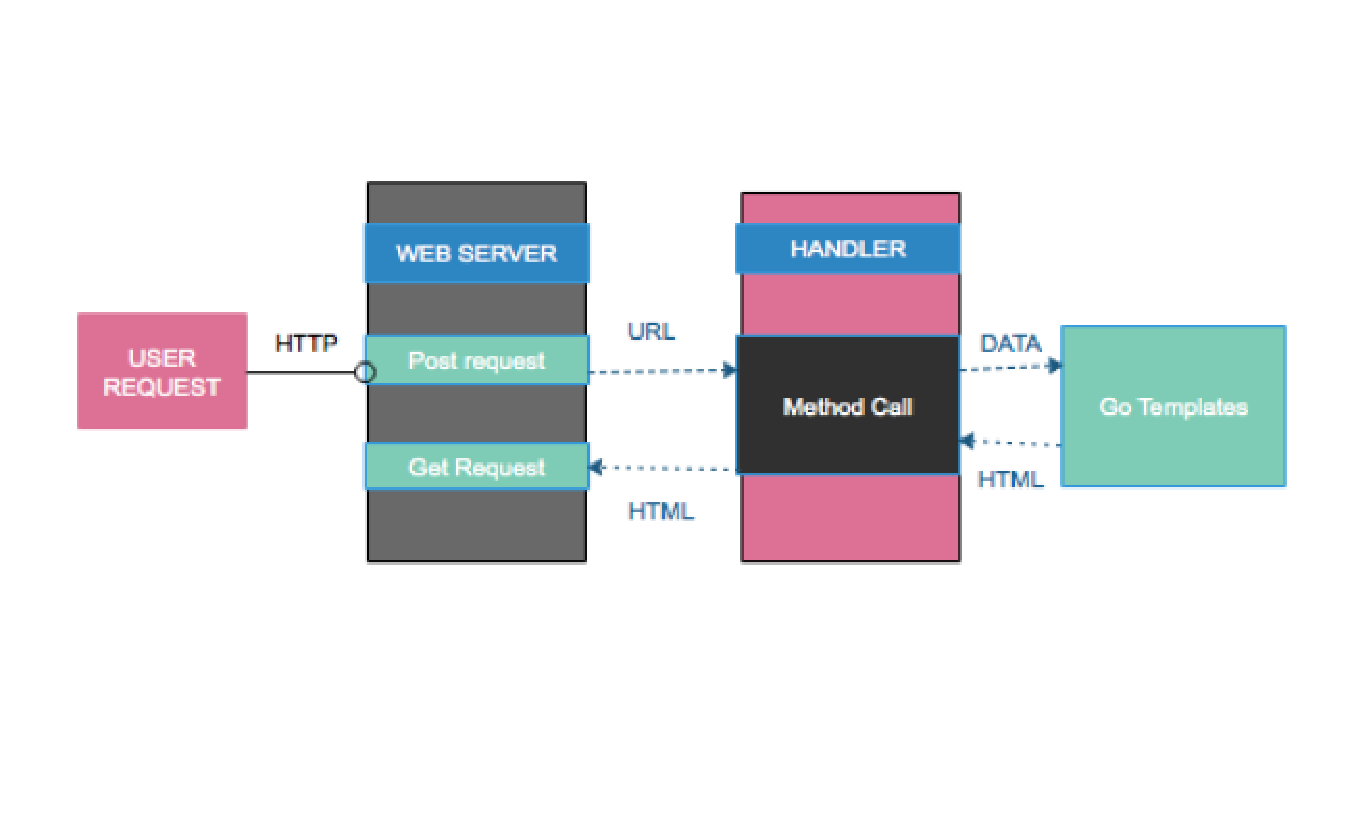
\includegraphics[width = \linewidth]{server1.eps}
\label{fig:Description of Server Activity} 
\caption{Server Activity Description}
\end{figure}

\pagebreak
\subsection{Database}
The database is another major component of this system, because it is provides storage and resource for the system. The data includes reservation records, machine details, disks, and NICs (network interface card) information. The database is designed with SQL model using Go programming language as the back end tech. SQL was used here as prototype because it is fast and easy to set up. We created a functional database system that address the specification of the software. 
The database scheme contains tables of machines, user record, reservation, NICs and disks.  One of the functions of the software is the ability to make reservations. \autoref{Databaseschema} shows a typical model of the database design.
\begin{figure}[h!]
\includegraphics[width = \linewidth]{database.eps}
\caption{Database design}
\label{Databaseschema} 
\end{figure}
\subsection{Data Flow}
The data flows from the user interface via the web server to the database. We used Go HTTP handlers to process data received from the HTML form to be stored in the database. The server initiates each method (function) when the HTTP handler sends a request. For example, when users search for list of information such as machine details, the request is sent through the server as a query, and the appropriate Go function is called to fetch the data from the designated database. Go HTTP handler uses a Request functon to call the server and  ResponseWriter to respond to the HTML request \cite{Gohttp}. The server uses ListenAndServe method to listen to incoming request and to call the requested method to handle the request. This process controls the sequence of data flow in the system. It controls data input, handling and output. This protocol helps the dynamic functionality on the user interface to perform in the system and also provides automatic command rather than manual query routine performed on command line. \autoref{sort} shows example of  handler function and \autoref{callsort} shows the registered function in the server.
\lstset{basicstyle=\footnotesize\ttfamily,breaklines=true}
\lstset{framextopmargin=50pt,frame=bottomline}
\begin{lstlisting}[caption=Sort Memory function in the handler, label=sort]
func (s Server) sortmPage(w http.ResponseWriter, r *http.Request) {
	s.logRequest(r)
	tname := "machines.html"
	t, err := getTemplate(tname)
	if err != nil {
		s.Error(err)
		templateError(w, tname, err)
		return
	}
	sortmemory,err := s.db.Sort_Memory()
		if err != nil {
		s.db.Error(err)
		renderError(w, "Error sorting",
			fmt.Sprintf("Unable to sort machines: ",
				err))
		return
	}
	t.Execute(w, sortmemory)
}
\end{lstlisting}

\lstset{basicstyle=\footnotesize\ttfamily,breaklines=true}
\lstset{framextopmargin=50pt,frame=bottomline}
\begin{lstlisting}[caption=Calling Sort Memory function, label=callsort]
http.HandleFunc("/machines/Sort_Memory/", server.sortmPage)
\end{lstlisting}


\chapter{Implementation}
\label{chap:ch4_abbr}
\label{chap:figtab}
\section{Review}
The software implementation showcases the functionality of all the requirements as described in section \ref{requirements}. This functionality includes the ability to input data and retrieve data through the system. We have accomplished this task by implementing the designed structure. This include the choice of tools used for the development and the design approach. It was implemented to demonstrate the realization of the proposed specifications.
\section{Implementation tools}
The user interface is implemented on the internet web browser using server port as web address. The web browser serves as the environment for testing the front-end (user interface) of the software, while the HTML template and Go library is used for development. The database was developed using the SQL model schema. The Go HTTP server provides connections between the front-end and back-end implementation. It servers as a channel for parsing request through user interface and database. These tools provided all the necessary components to address the requirements for this software. 
\section{Program Structure} \label{Programstructure}
The Go programming language has a development structure that is categorized into packages, see \autoref{programpack}. The packages contains a group of program file with dependencies that links them together. For this software design, we have written two main package to actualize the development goal. In addition to other people's works in these packages, I have added more files with numerous methods and functions of couple or more thousand lines of SQLite, Go and HTML codes that improves the system requirements. These packages includes:
\begin{description}
\item[$\bullet$]Database package 
\item[$\bullet$]HTTP package 
\end{description}

The database package contains all the Go files with database related struct. The Go objects represent the same data as in the database. And each Go struct depends on this package as the object-relational mapping tool (ORM) between other struct and database resources. The HTTP package also contain some Go file relates to the user interface (for example the function handler) and HTML files. The HTML files contains several templates for the web interface content and elements. These files depends on the GO HTTP package for serving web contents and post requests. \autoref{programpack} describes the list of files in each package.
\pagebreak
\begin{table}[h!]
  \centering
  \begin{tabular}{ccc}
    \hline
    No & Package & File\\
   \hline
    1 &Database (pkg)& machine.go\\
       &&reservation.go\\
      &&disk.go\\
      &&user.go\\
      &&nic.go\\
    \hline
    2 &HTTP (pkg)& handler.go\\
    &&server.go\\
    &&HTML templates\\
    \hline
  \end{tabular}
  \caption{Program packages}
  \label{programpack}
\end{table}

\section{List of Struct and Methods}
\autoref{sm} shows the class diagram of the list of struct and methods with their relationships with others. It shows the group of methods that perform the tasks specified in the software requirement in our design.
\begin{figure}[h!]
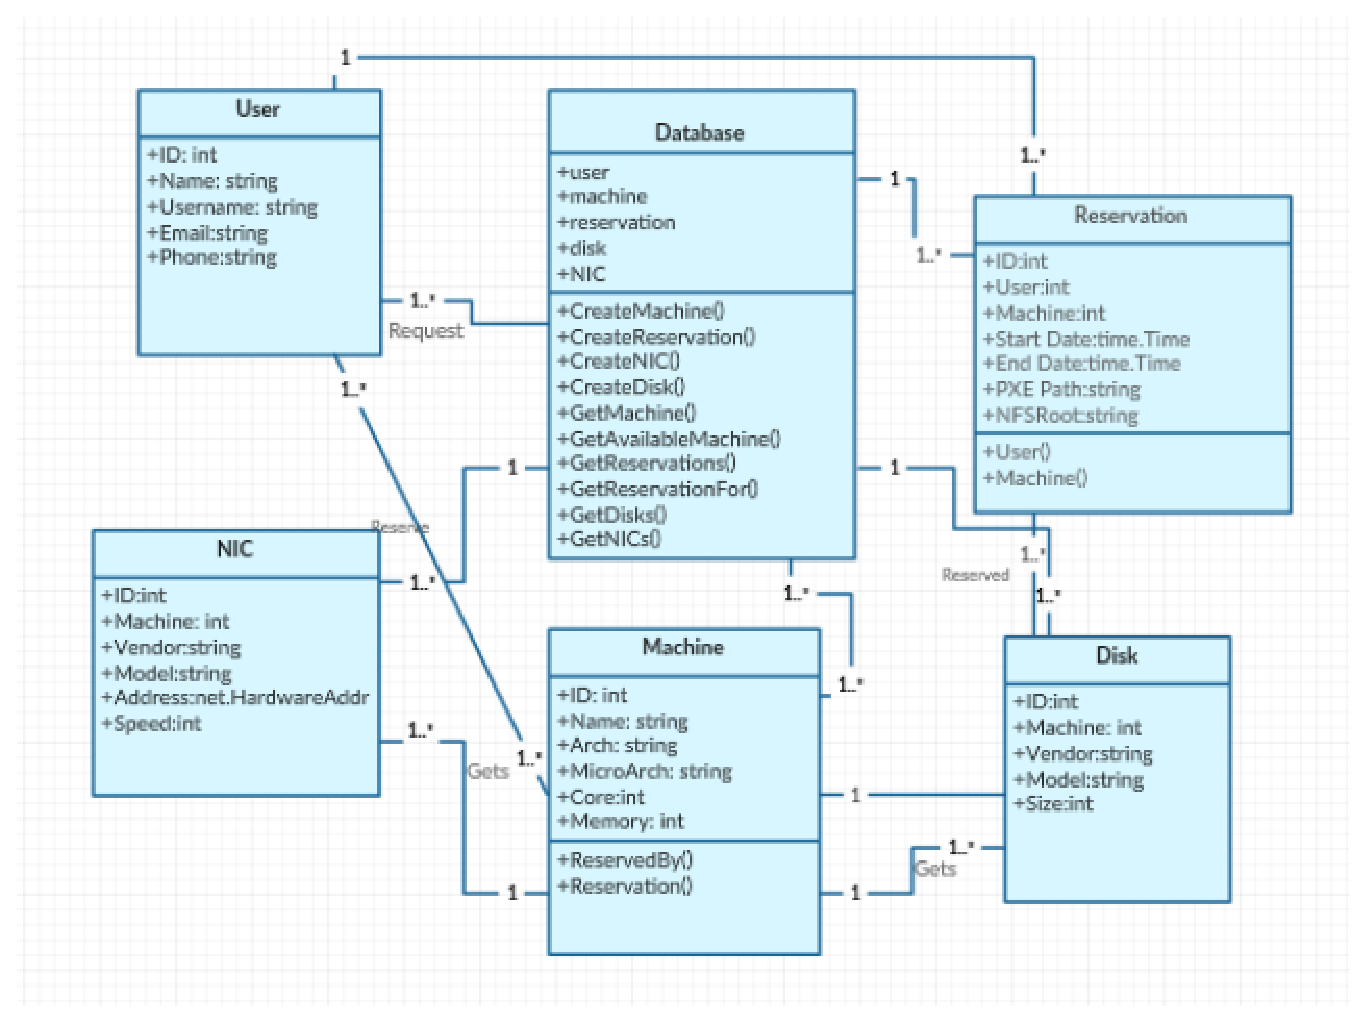
\includegraphics[width = \linewidth]{methods.eps}
\caption{Class Diagram showing struct and method relationships}
\label{sm} 
\end{figure}
\pagebreak
\section{Description of Methods}
\section*{Adding Machines to the system}
Adding machines and other devices to the system is one of the software requirements in section \ref{addmachines}. On the user interface, the software provides a text field and forms where users can enter details of machines to be saved as data in the database. The InitMachine method create a new database schema with defined table fields where data is stored. When the user submits a Add Machine form, the InitMachine create the database schema where the machine details is stored. It uses type (Machine) fields as argument for creating the schema fields. \autoref{Initializingdatabase} is the code listing for creating database:
\lstset{basicstyle=\footnotesize\ttfamily,breaklines=true}
\lstset{framextopmargin=50pt,frame=bottomline}
\begin{lstlisting}[caption=Creating Database for machine, label=Initializingdatabase]
func initMachines(tx *sql.Tx) error {
	_, err := tx.Exec(`
	CREATE TABLE Machines(
		...........
	);`)
	return err
}
\end{lstlisting}
The CreateMachine method is responsible for parsing the data to the database schema. It uses the SQLite INSERT query to parse a give data using the arguments to the database. When the user submit a form (AddMachine), the Go HTTP handler process this form by converting the plan text to a form data according to their data types defined in the schema, and then call the CreateMachine to insert this data to the database. \autoref{Addingmachine2} shows the code list.
\begin{lstlisting}[caption=Adding machines details, label=Addingmachine2]
func (d DB) CreateMachine(name string, arch string,
	microarch string, cores int, memoryGB int) error {
	_, err := d.sql.Exec(`
			INSERT INTO Machines(name, arch, microarch,
			 cores, memory)
			VALUES (
				//field values
			)`,
		name, arch, microarch, cores, memoryGB)
	return err
}
\end{lstlisting}

\section*{Making a Reservation}
The reservation process is similar to creating a machine but here it requires the User ID and Machine ID as foreign keys in creating the database schema \ref{makereserve}. The User ID is used for selecting the user making the reservation, and Machine ID for selecting the machine to be reserved. On the web interface (reservation page), the form has a drop down list where users can select their user name and the machine they want to reserve. When users open the reservation page to create new reservation, the HTML form use the post request to get list of machines and user name on the drop-down list.
PSEUDOCODE:
\begin{enumerate}
\item Input reservation values in the field.
\item Select machine id from the list where machine name is chosen.
\item Select user id from the list of user where name is chosen.
\item Insert all the values to reservation table and return.
\end{enumerate}
\begin{lstlisting}[caption=Storing Reservation details, label=Adding reservation]
	_, err := d.sql.Exec(`
			INSERT INTO Reservations(machine,user,start,end,
			pxepath,nfsroot)
			VALUES (
				(SELECT id from Machines where name=?),
				(SELECT id from Users where username=?),
				//other fields
			)`,
\end{lstlisting}

To make a reservation, users select their user name and a machine from the drop down list which is loaded by GetMachine and GetUser method. The selection query gets the User ID and the Machine ID of the selected user name and machine as foreign key to the reservation database schema. Also, start and end time/date of the reservation is entered on the text field , and this plain text is formatted to match the database using a time package in Go library. After submitting the form, the Go HTTP handler handles the Insert query by taking all the argument values and saving them to database. 
\section*{Checking Available Machines}
The user can search the inventory for specific imformation. One of the example is the ability to search for available machines in the system as one of the requirement \ref{searchinventory}. Available machines are those machines that are free for a certain period. This feature helps users to get list of machine free to be reserved. In this process of checking available machine, the user enters a specific start date and end date in the provided text feild, and submits the query. After submiting the query, the HTTP handler processes this request, and the server calls the GetAvailableMachine method to fetch this request from the database. In this method, we used a SQLite JOIN sub query to combine the machine and reservation database table. This combination logic allows the query to scan through both table rows using reservationID and machineID to indentify the machines that are not reserved for that time range the user entered. The logic contains SQL WHERE, OR and AND operator to perform comparisons between reservation dates and time. \cite{ANDOR}The AND operator is used to allow multiple conditions in the statement,  the OR operator is used to combine condition that are true, and the WHERE clause is used to specify condition while fetching data from database\cite{WHEREclause}. 
\autoref{SAM} shows the function and query for this operation.
PSEUDOCODE:
\begin{enumerate}
\item Set the function arguments.
\item Query rows in machine table and select where id is not reserved.
\item Query rows in reservation and select machine where reserved outside of the search dates START and END date. 
\item Combine the values from the two tables.
\item Assign the selected values to the row and return the values.
\item Return values selected 
\end{enumerate}

\begin{lstlisting}[caption=Searching available, label=SAM]
func(d DB) Filter_M_By_Dates(from time.Time, to time.Time) ([]Machine, error){

         rows, err := d.sql.Query(`
		SELECT m.id, name, arch, microarch, cores, memory
		FROM Machines m
		WHERE m.id NOT IN (SELECT r.machine FROM Reservations r
		WHERE (? BETWEEN r.start AND r.end)
		OR (? BETWEEN r.start AND r.end)
		AND  ( r.start BETWEEN ? AND ?) OR (r.end BETWEEN ? AND ?)
	
	); `, from, to, from, to, from, to)
\end{lstlisting}
\section*{Updating Machines details}
As part of the software requirements, users can change the information stored in the database. This is done on the web interface using text box that is attached to every field with that requirement. Example is updating the information of a particular computer or disks when the hardware is upgraded. In this case, the UpdateMachine method performs this action by using the SQLite update query. This update query opens the database schema of the machine and replaces the existing data with a new one.
\autoref{Updatefunction} code listing shows the update function:
\begin{lstlisting}[caption=Function for Updating data, label=Updatefunction]

	_, err := d.sql.Exec(`
			UPDATE Machines
			SET arch = ?, microarch = ?, cores = ?, memory = ?
			WHERE `+row+` = id

	`,arch, microarch, cores, memory)

\end{lstlisting}
\section{Get methods}
The Get function is a method used for fetching list of machines and other devices stored in the database. Each time the user opens the web interface, the HTTP handler send server a request and server calls the GetMachines method to fetch the data from database. This information is listed in the inventory on the web interface through the HTTP Response-Writer. The Get methods uses the SQLite selection query to scan through the database and select the required data.  Another usage for this Get method is fetching the details of a machine when the user click on a particular machine. It uses a SELECT query and WHERE condition in the logic, to specify the machine clicked used its unique ID. This methods is applicable in other struct (type) such as, Disks, NICs and Reservations. 
 
\section{Problems Encountered}
During the implementations, we encountered problems such as formatting plain text to database data types. For example, some functions can parse a plain text as they are to the database, but in some cases where the values have a different data type (eg. Hardware Mac-address data type), this data cant be store as plain text.  So this problem was solved by importing special functions from the Go library to support those data types. Another issue encountered is trying to combine two database table for search queries. This problem was mostly encountered in the implementation of search query, where two tables were combined for comparing different data.  We solved this query problem by using SQL JOIN function, which normally link different data from multiple database table by scanning through them. With this problem solved, it helped us during the implementation to add more functionality to the user interface without having further error prone situations.




\chapter{Evaluations} 
\label{chap:refs}
\label{chap:ch5_abbr}
\section{Test cases}
We have evaluated this software by testing different functionality as specified in the requirement. This was achieved by creating multiple cases that proves the performance of the software. This evaluation was performed in real time and directly online. We have included images and table showing the test cases and results. 
\section*{Checking Available Machines}
In the software specification, it is designed to have search option on the user interface. One of this search requirement is to check for available machines (unreserved machines). In the below table is list of machines reserved for different date. The test is to enter a search query with a specific date interval and ask the software to provide any machine available withing that date.

\begin{table}[h!]
  \centering
  \label{tab:table1}
  \begin{tabular}{l|c||c||c||c||c||c||r}
    No & Machines & Aug & Sep & Oct & Nov & Dec & Jan \\
    \hline
    1 &Machine A & free & free & free & free & free & free\\
    2 &Machine B & free & free & free & 1st to 30th & free & free\\
    3 &Machine C & 17th - & - & - & 24 & free & free\\
    4 &Machine D & 25 & - & 25 & free & free & free\\
    5 &Machine E & free & free & 1st to 31st & free & free & free\\
    6 &Machine F & free & free & free & free & 2nd to 31st & free\\
  \end{tabular}
  \caption{List of Reservations}
\end{table}

\begin{table}[h!]
  \centering
  \label{tab:table1}
  \begin{tabular}{l|c||r}
    No & Date: start --- end & Available machines\\
    \hline
    1 &12-08-2017 to 30-08-2017  & A B E F \\
    2 &17-08-2017 to 24-08-2017  & A B D E F\\
    3 &01-08-2017 to 05-10-2017  & A B F \\
    4 &05-08-2017 to 10-08-2017  & A F \\
    5 &01-08-2017 to 30-08-2017  & A D E  \\
    6 &01-01-2018 to 30-01-2018  & A B C D E F \\
  \end{tabular}
  \caption{test 1}
\end{table}

\begin{table}[h!]
  \centering
  \label{tab:table1}
  \begin{tabular}{l|c||r}
    No & Date: start --- end & Available machines\\
    \hline
    1 &01-08-2017 to 01-01-2018  & A \\
    2 &01-08-2017 to 15-11-2017  & A F\\
    3 &01-12-2017 to 30-01-2018  & B C A D E \\
    4 &30-11-2017 to 30-12-2017  & A  C D E\\
    5 &02-10-2017 to 02-08-2017  & A  D E \\
  \end{tabular}
  \caption{test 2}
\end{table}
\pagebreak

\section*{Reserving a machine}
Reserving machine is another requirement we have implemented in this software. This is the process where users choose and reserve a machine for definite time and date. When a reservation is made, the details of the reservation appears under the machine being reserved. Figure \ref{fig:reserve} shows the evaluating of this function, where we put details of reservation, by selecting a user name, machine and inserting start and end time/date. After submitting with the reserve button, the it appears on the inventory with other reservations list. 
\begin{figure}[h]
  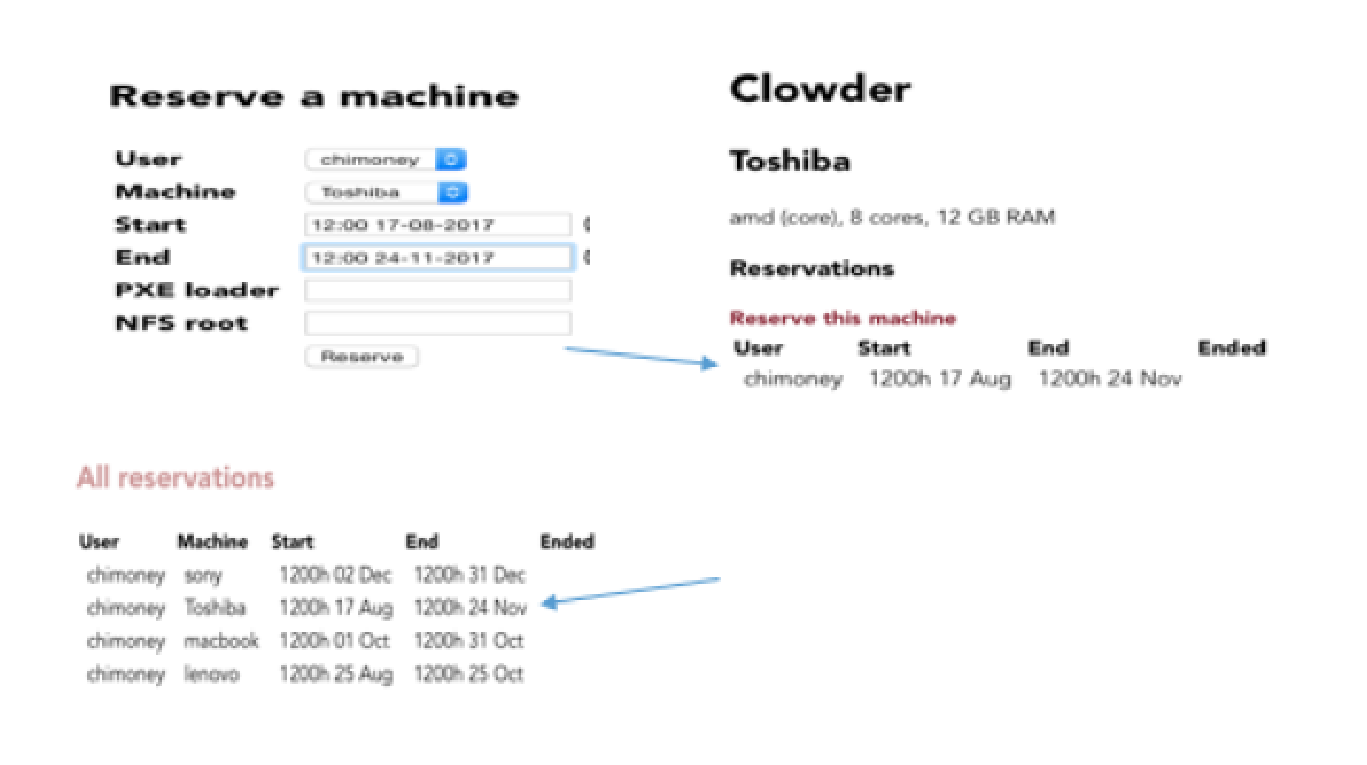
\includegraphics[width=\linewidth]{reserve.eps}
  \label{fig:reserve}
  \caption{Reservation function}
\end{figure}

\begin{figure}
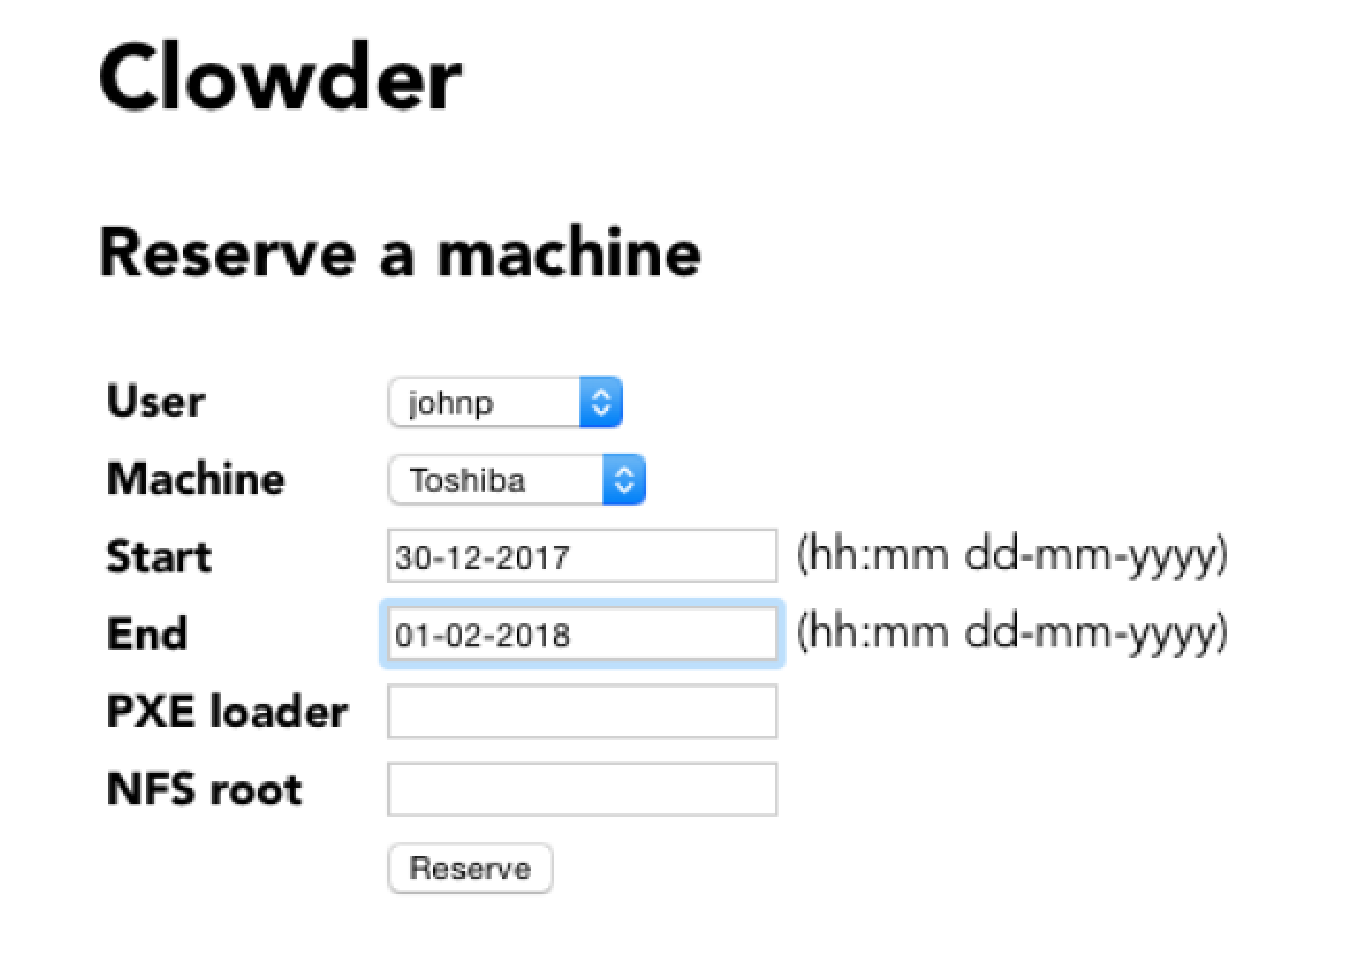
\includegraphics[width=\linewidth]{dateformat1.eps}
\caption{reserving with wrong date}
\end{figure}

\begin{figure}
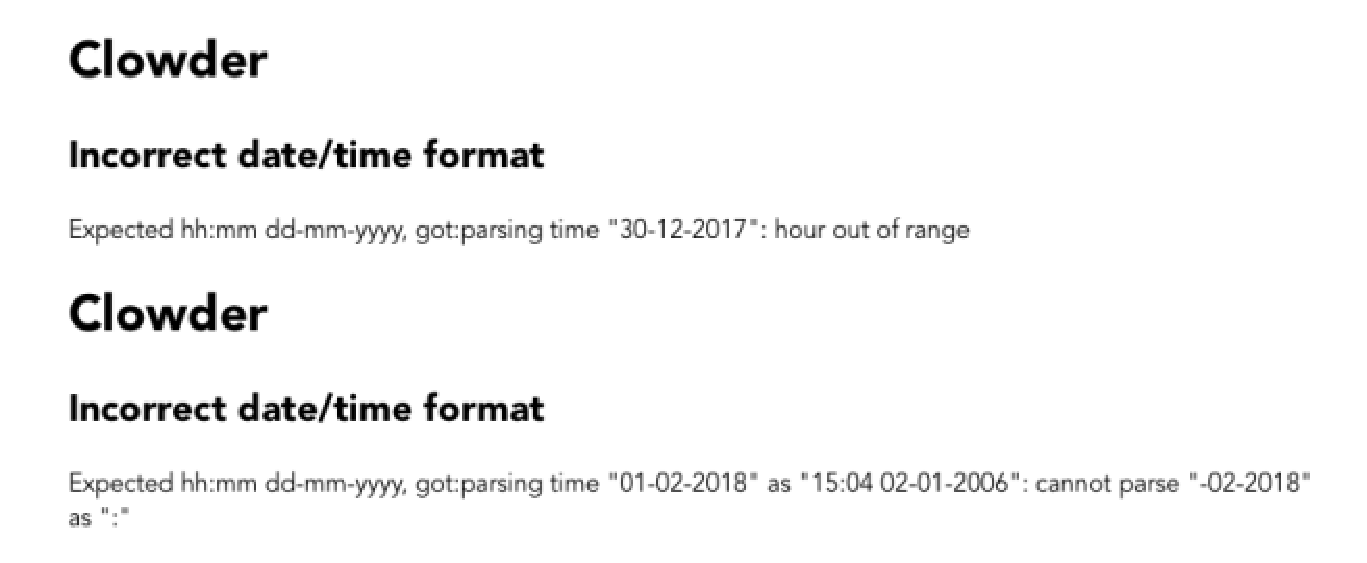
\includegraphics[width=\linewidth]{dateformat2.eps}
\caption{Error message}
\end{figure}

\begin{figure}
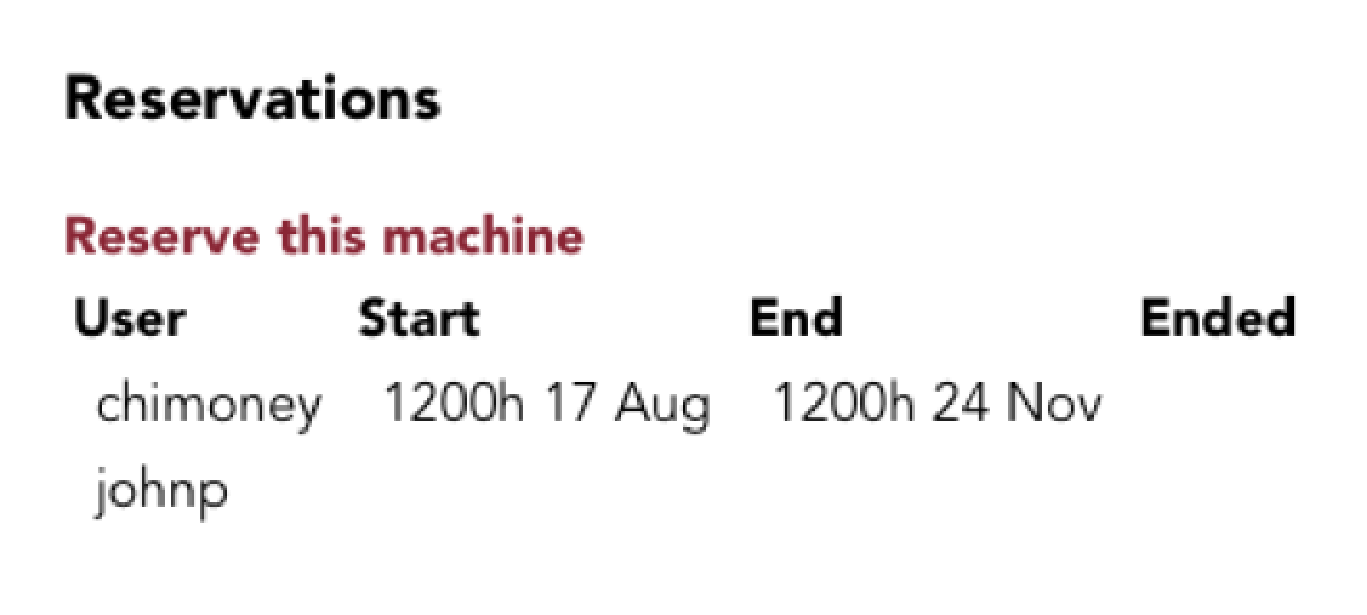
\includegraphics[width=\linewidth]{dateformat3.eps}
\caption{Invalid reservation}
\end{figure}
\pagebreak

\section*{Updating a machine}
Update functionality allow users to change the details of a machine already stored in the database. This is to enable them update the information about each machine as needed when ever there is an upgrade in the system. We have tested this functionality by changing the entire information of a machine listed in the inventory. Figure \ref{fig:reserve}  shows an example of this test case.
\begin{figure}[h]
  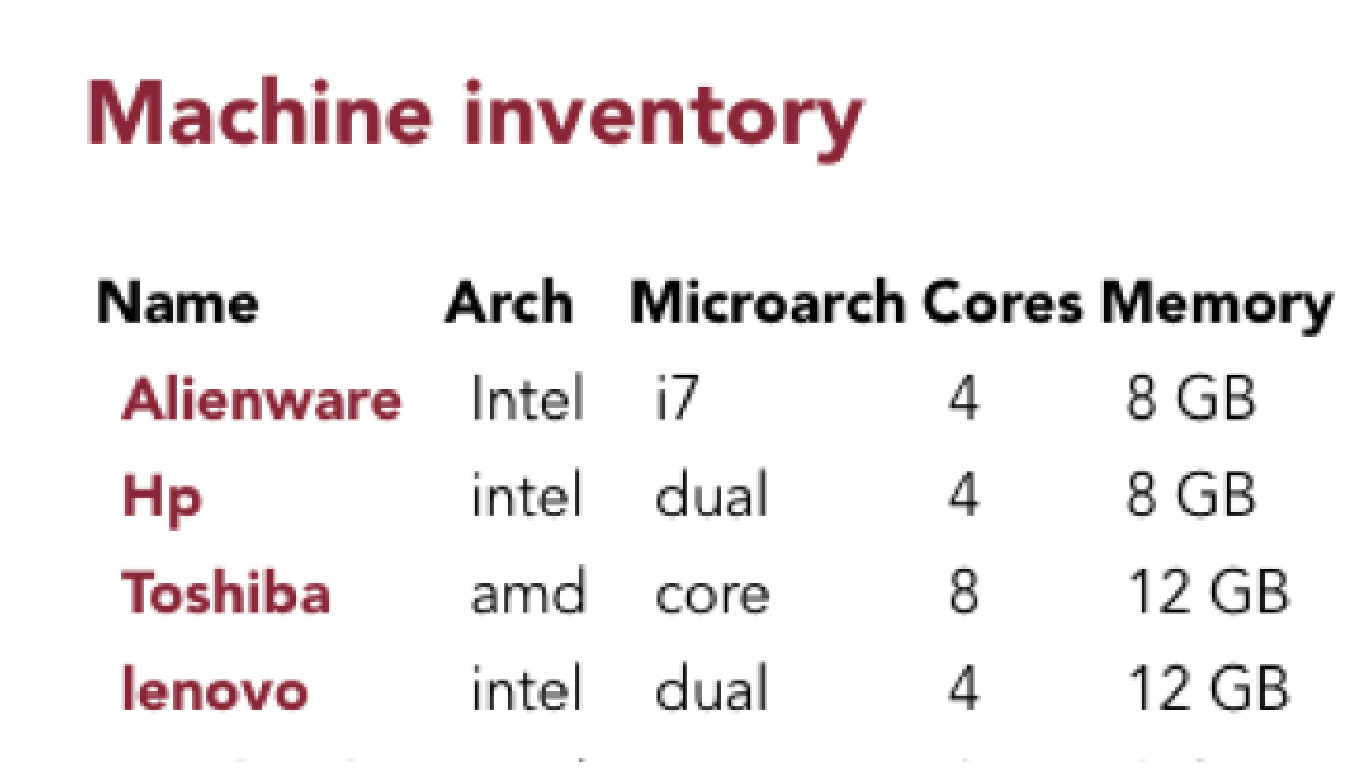
\includegraphics[width=\linewidth]{update.eps}
  \label{fig:reserve}
  \caption{Before update}
\end{figure}
\begin{figure}[h]
  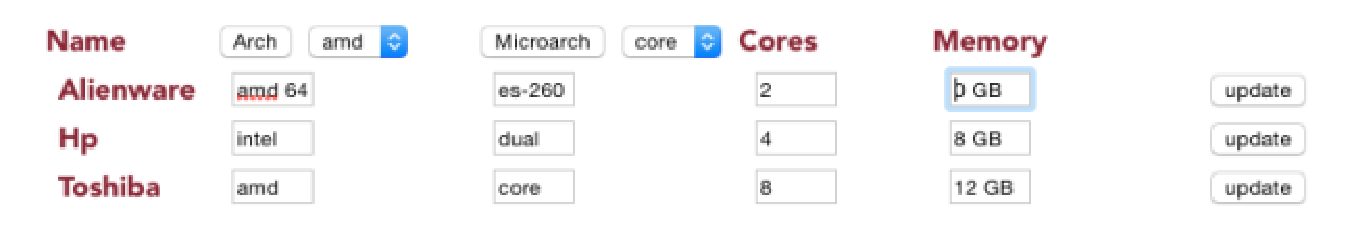
\includegraphics[width=\linewidth]{change.eps}
  \label{fig:reserve}
  \caption{Editing machine details}
\end{figure}
\begin{figure}[h]
  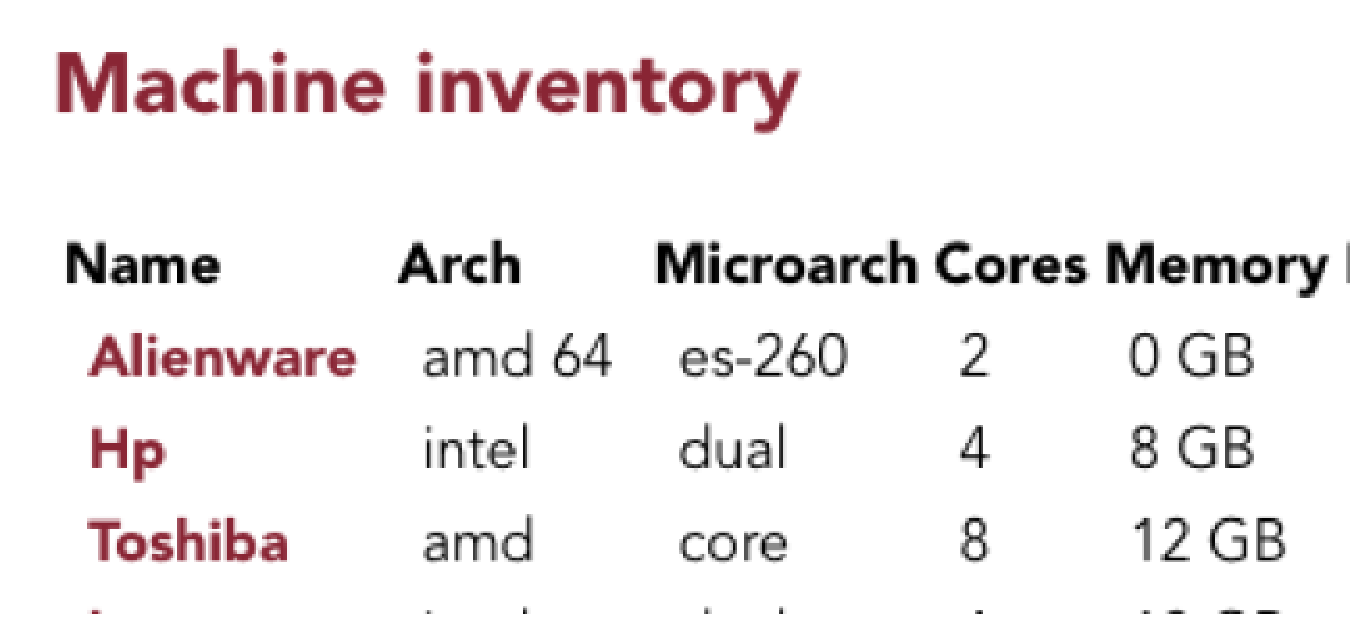
\includegraphics[width=\linewidth]{update2.eps}
  \label{fig:reserve}
  \caption{Updated machine properties}
\end{figure}
\pagebreak

\section*{Filtering inventory}
This functionality helps user to filter the inventory using the context of desired information. User is able to filter the machines inventory with memory size. The size range is inserted in the search to get the list of machines that fall within the range. When the button is clicked, the  server returns the list of machine that falls in the range. Another type of filtering is the the drop list filter. This type has a drop down menu user select a context option to search for. For example, user can filter the machine inventory by selecting type OS micro-architecture and architect.
\begin{figure}[h]
  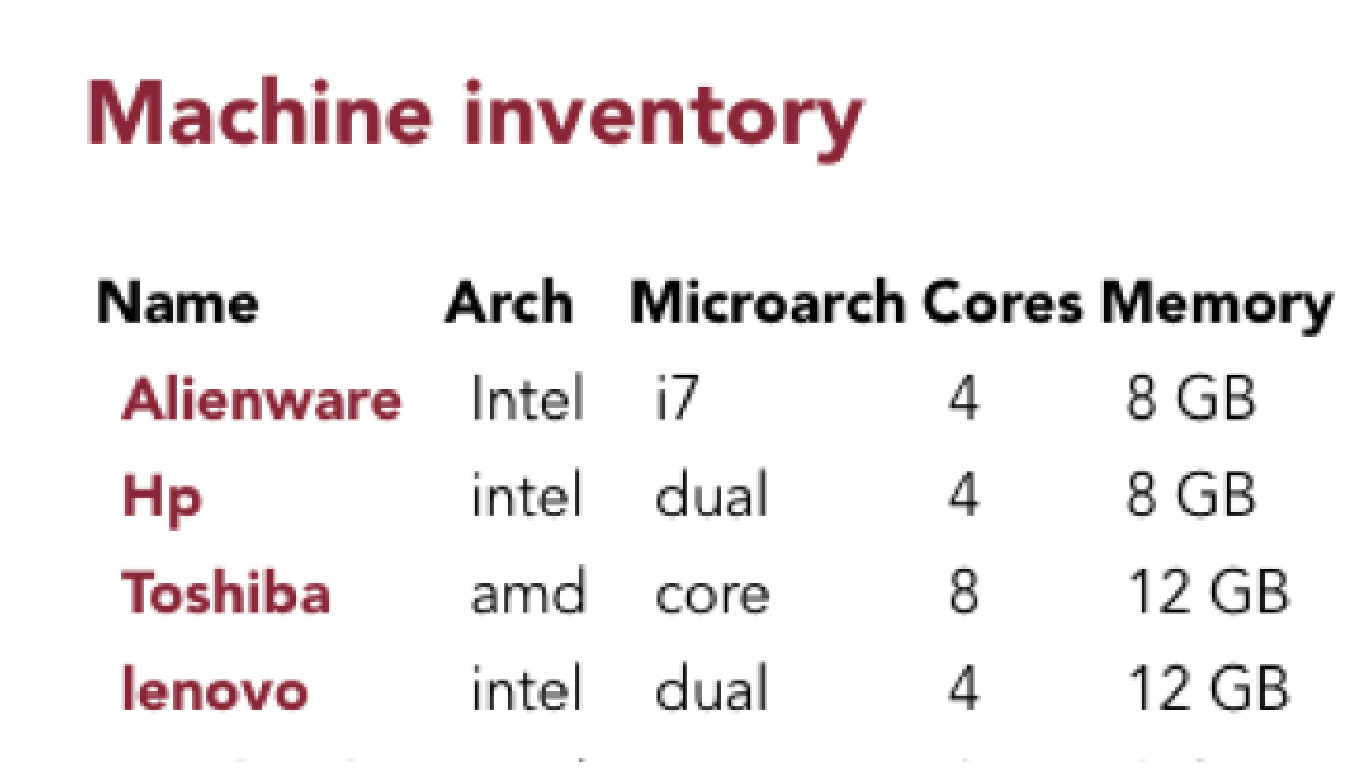
\includegraphics[width=\linewidth]{update.eps}
  \label{fig:reserve}
  \caption{Reservation function}
\end{figure}
\pagebreak

\section{Evaluations}
During the testing of this software, we have evaluated the performance by doing a general evaluation on events of the requirements be recording the speed of network request, layout and rendering of interface content, and theirs scripts.  Below are the evaluations:
\begin{figure}[h]
 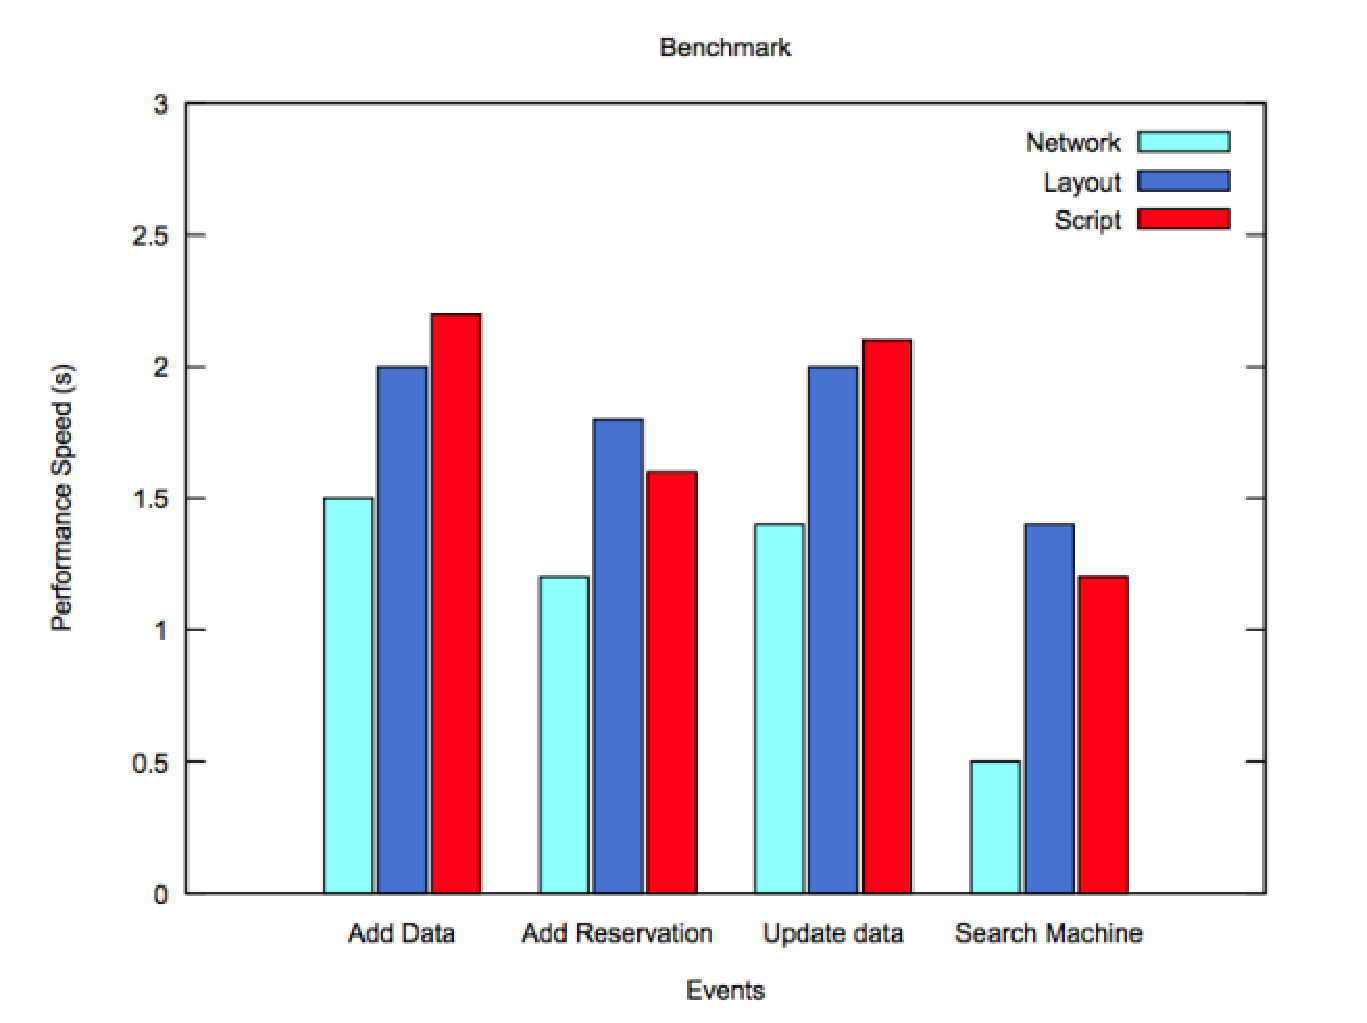
\includegraphics[width=\linewidth]{evaluation.eps}
  \caption{General Evaluation }
\end{figure}
\begin{figure}[h]
 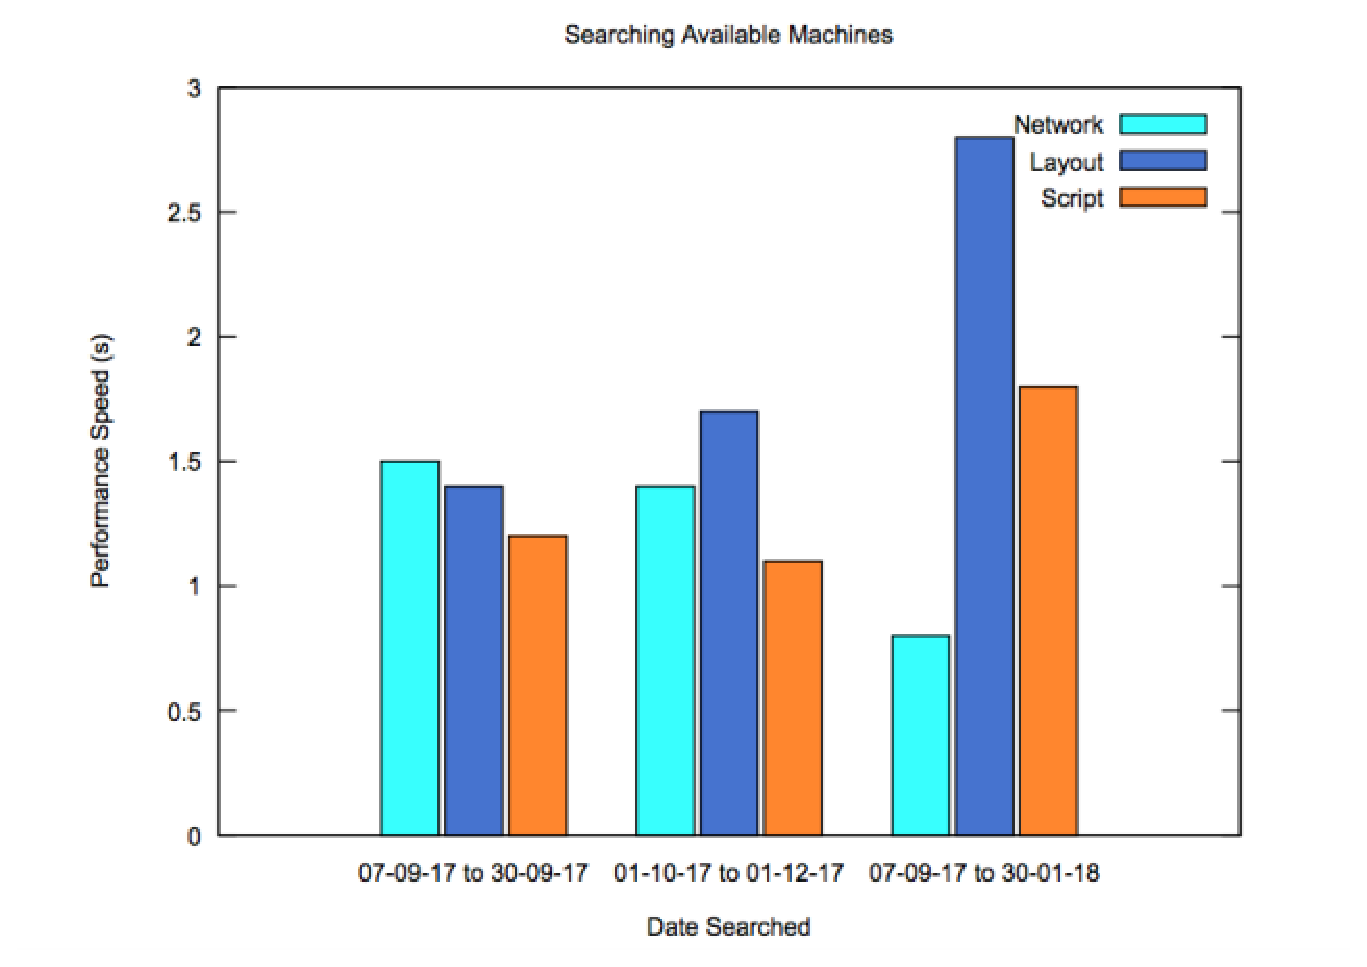
\includegraphics[width=\linewidth]{evaluation2.eps}
  \caption{Search Available Machines}
\end{figure}

\chapter{Conclusion}
\label{chap:conclusions}

The need to complete the clowder system which was design to manage test machines has been accomplished by addressing the issues of system managemnt and accessibility. It was required to have a flexible user interface for dynamic accessibility, and a functional database system for storage and management. This issues has been resolved by designing a frontend and extended backend  software that provides the required functionality for the user interface and the database. We have created a web interface where users can communicate with the test by sending request via HTTP protocol. This web interface contains the required functionality for making reservations, updating machine details and viewing the inventory and generally resolve the issue of user accessibilty. Also, as part of the requirement to complete the Clowder system, we created a SQL database for storing and retrieving data. This database enables the clowder system to manage the access and users activity on the test machines by storing their details and recording all reservations made by users. The the database we have created has the ability to plug in a DHCP server which provides network between the Clowder and the test machines. All these factors has made is easier for researchers to run their test on the machines without conflict and lost of data. 

\addcontentsline{toc}{chapter}{Bibliography}
\bibliographystyle{ieeetr}
\nocite{*}
\bibliography{ref}

\begin{appendices}
\chapter{Appendix A}
\autoref{randscript1} shows the basic python script used for random generated machines and reservations.
\lstset{basicstyle=\footnotesize\ttfamily,breaklines=true}
\lstset{framextopmargin=50pt,frame=bottomline}
\begin{lstlisting}[caption=Script for generated data, label=randscript1]
#!/usr/bin/python
# -*- coding: utf-8 -*-

import sqlite3 as lite
import sys
import datetime
import random
from datetime import date

con = lite.connect('clowder.db')

with con:

    cur = con.cursor()

    cur.execute("INSERT INTO Machines WITH RECURSIVE mch(id, name, arch, microarch, cores, memory)AS(SELECT random(),abs(random()% ),abs(random()%),abs(random()%),abs(random()%),abs(random() %)UNION ALL SELECT random(),abs(random() %),abs(random()%),abs(random()%),abs(random()%),abs(random()%)FROM mch LIMIT 0 ) select * from mch;")
    
     cur.execute("INSERT INTO Reservations WITH RECURSIVE res(id,user,machine,start,end,ended,pxepath,nfsroot)AS(SELECT random(),(SELECT users.id from Users),(SELECT machines.id FROM Machines),abs(random() (strftime('%s','2017-10-31 23:59'))),strftime('%s','2017-01-01 00:00') + abs(random()% (strftime('%s','2018-01-31 23:59') - strftime('%s','2017-01-01 00:00'))),NULL,abs(random()%),abs(random()%)UNION ALL SELECT random(),(SELECT users.id from Users),(SELECT machines.id FROM Machines),abs(random()% (strftime('%s','2017-01-31 23:59'))),strftime('%s','2017-01-01 00:00') + abs(random()% (strftime('%s','2018-01-31 23:59') - strftime('%s','2017-01-01 00:00'))),NULL,abs(random()%),abs(random()%)FROM res LIMIT 0 )select * from res;")
if con:
    con.close()

\end{lstlisting}
\chapter{Appendix B}
Random generated number of machine and reservations for \autoref{mandr}.
\begin{table}[h!]
  \label{tab:Scattered plot data}
  \begin{tabular}{l|c||r}
    No & Number of Machines & Number of Reservations\\
    \hline
    1 &5 &10  \\
    2 &10 &5 \\
    3 & 15&550  \\
    4 & 20&35  \\
    5 & 50&180  \\
    6 &100 &670 \\
    7&150&120 \\
    8&250&1000 \\
    9&500&50 \\
    10&1000&180 \\
    11&2000&1600 \\
  \end{tabular}
  \caption{Scattered plot data}
\end{table}

The following table shows the data generated from Network and Layout time of the software performance as  shown in \autoref{available}, \autoref{addmachine} and \autoref{addreservation}.
\begin{table}[h!]
\label{tab:availabledata}
\begin{tabular}{l|c||r}
No of Machines & Network Time(ms) & Layout Time(ms)\\
\hline
30&85&35 \\
65&180&65 \\
125&420&180 \\
250&991&248 \\
500&3100&460 \\
1000&9000&860 \\
2000&18000&1680 \\ 
\end{tabular}
\end{table}

\begin{table}[h!]
\label{tab:availabledata}
\begin{tabular}{l|c||r}
No of Machines & Network Time(ms) & layout Time(ms)\\
\hline
30&62&25 \\
65&134&43 \\
125&280&80 \\
250&571&170 \\
500&1000&380 \\
1000&1700&810 \\
2000&2550&1800 \\ 
\end{tabular}
\end{table}

\begin{table}[h!]
\label{tab:availabledata}
\begin{tabular}{l|c||r}
No of Machines & Network Time(ms)& Layout Time(ms)\\
\hline
30&147&37 \\
65&231&52 \\
125&445&74 \\
250&870&120 \\
500&1300&340 \\
1000&2800&447 \\
2000&3960&830 \\ 
\end{tabular}
\end{table}
\end{appendices}


\end{document}
